\documentclass[12pt]{article}
\usepackage[utf8]{inputenc}
\pagenumbering{arabic}
\usepackage{graphicx}
\usepackage{amstext}
\usepackage[usenames, dvipsnames]{color}
\graphicspath{ {images/} }


\begin{document}

\begin{titlepage}
    \begin{center}
    \begin{figure}
        \centering
        
\includegraphics[scale=0.2]{logoPolimi.png}
        \vspace{1.5cm}
    \end{figure}

    \Huge\textbf{Software Engineering 2 Project - Travlendar+}
    \rule{12cm}{0.5pt}
    \Huge\textbf{RASD - Requirement Analysis and Specification Document}
    \today
    \end{center}
    
    \vspace{3cm}
    
    \begin{flushleft}
        \LARGE\textbf{Authors: }
        \newline\newline
        \Large\texttt{}{Francisco Cristóvão \\ Samsom Beyene}
    \end{flushleft}



\end{titlepage}

\newpage
  \tableofcontents
\newpage

\section{Introduction}

\subsection{Purpose}

The main goal of this project is to create a calendar-based application which provides the user a flexible and fully-featured calendar support that considers the travel time between meetings. With this in mind, the application will:
\begin{itemize}
\item compute and account for travel time between appointments, and prevent conflicts between them
\item support the user in his/her travels, adding automatically the travel time to the calendar between meetings, and suggesting the best travel option based on the available time
\end{itemize}

\subsection{Scope}
Travlendar+ is a calendar-based application that provides the user a convenient way of organizing his/her daily schedule, maximizing its productiveness and minimizing the worthless time of his/her day. This application was not only thought for the regular businessman/businesswoman, who travel in between meetings the whole day and have no time to spare, but also for the parents with a more regular daily schedule, who just want to get the best of their time while being able to pick their kids from school and take them to other activities, always being on time.
Of course the system will fully support the features of a regular calendar application (booking of appointments in a specific time and location), but in a "smart" way, being able to detect and warn the user if a new appointment is not feasible because it has a conflict (the start of it doesn't allow the needed travel time after the end of the last appointment). The application is meant to be used in the City of Milan, and so it will take advantage of the wide range of travel means and services already existing in the city, from public transports to shared bikes and cars. With the information gathered from those services, it will be able to suggest the best travel mean for the user to move between appointments, based on the available travel time, total cost, current weather and even user preferences.


\subsection{Definitions, Acronyms, Abbreviations}

\subsection{Revision History}

\subsection{Reference Documents}
Assignment document: Mandatory Project Assignments.pdf

\subsection{Document Structure}
Other than this introductory chapter, this RASD is organized in five more chapters. Chapter two is meant to provide an overview of the systems functionalities, the type of users it is meant for and the different kinds of interactions it contemplates, not only with the users themselves, but also with other systems. Some of the systems requirements are also slightly discussed in this chapter, even though they’ll be analysed in the following chapter. In the third chapter (as mentioned above) the systems requirements, attributes and constraints are analysed and discussed with the appropriate detail and depth, specifying exactly how they should be.
The fourth chapter deals with the formal analysis of the system using and Alloy model. It includes the Alloy model of the system, with a brief discussion on its purpose and on the relevance of using Alloy as a tool to validate our solution, given the problem we had to solve.
In the fifth chapter the effort spent by each of the group members is described by specifying the number of hours each member of the group worked on the development of this document.

\section{Overall Description}

\subsection{Product Perspective}
The application will need to communicate to both Public transport system , bike or car sharing system of the city and Google maps API to find the exact status of available (active) types of transportation with their corresponding locations. These information’s helps the application to exactly locate the position of the user and meeting place so that it can assign the travel means with its calculated time. In addition, the application also retrieves the weather conditions while making some decisions. 
Since this application is data centric product it will need somewhere to store the schedules. For that a database is used. So the mobile application will communicate with the database (probably distributed database) to add, modify or view the schedule. All the database communication will go over the Internet.

    \begin{figure}[ht]
        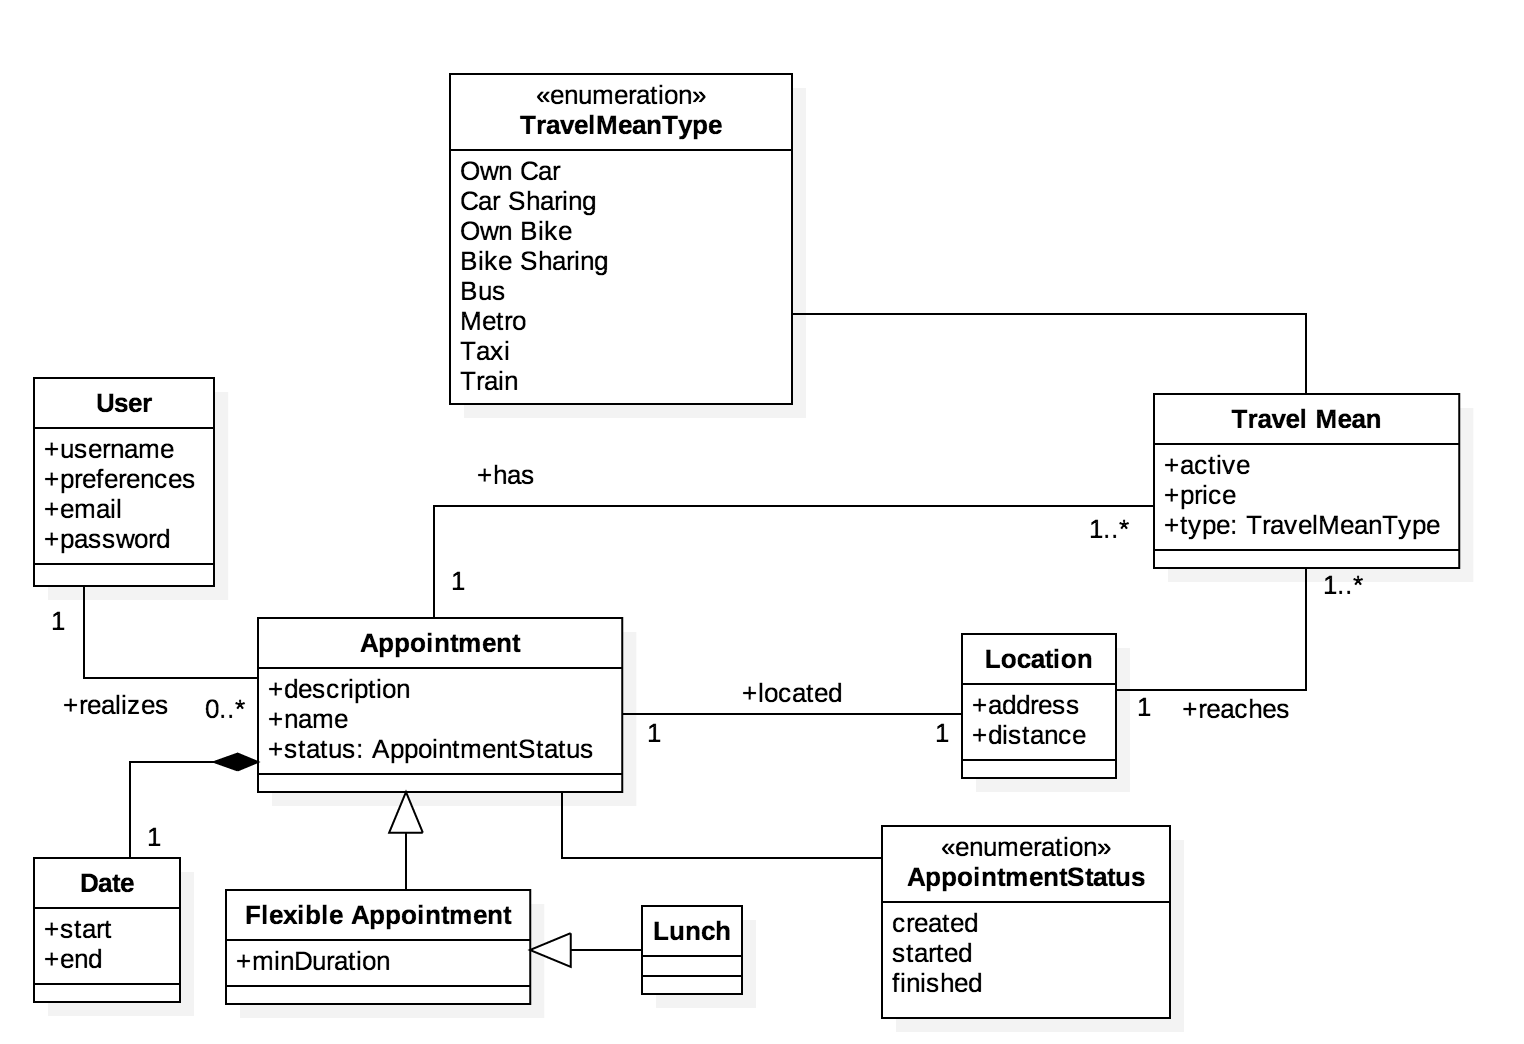
\includegraphics[scale=0.52]{domainModel.png}
        \caption{Class Diagram of the domain}
    \label{fig:domainModel}
    \end{figure}
    
\subsection{Product Functions}

\subsection{User Characteristics}

\subsection{Assumptions, dependencies and constraints}
[D1] The username must be unique.  
[D2] The system will have access to the phone GPS functionality.

\section{Specific Requirements}

\subsection{External Interface Requirements}

\subsubsection{User Interfaces}

\subsubsection{Hardware Interfaces}
In the first release no Hardware Interfaces will be necessary, since the system doesn't need to interact physically with other systems.

\subsubsection{Software Interfaces}
Given the wide range of features the system offers, it will need to have several software interfaces. There has to be a way of storing all the user-related data (mainly login and preferences data). In that sense, the system will use a \textbf{MySQL API} to connect with a MySQL database server, where all the app data will be stored.\\
The system will also need different kinds of information about the users location and its surrounding, in order to compute the travel time between appointments. To support this functionality, the system will use \textbf{Google Maps Geolocation API} and \textbf{Google Maps API}. The first one will provide information about the user exact location and the second one will provide the real-time information about maps and traffic, and allow it to calculate the best route between two different appointments.\\
To have access to the current weather, the system will use \textbf{AccuWeather API}, which will provide information about the current weather either where the user is or where the user is going.
At last, the system also needs to get all sorts of information from many different travel means. In order to get this information, it will have a software interface with \textbf{ATM Milano} (public transport schedule and routes), \textbf{Drive Now API} (for the car sharing system) and \textbf{Ofo API} (for the bike sharing system).



\subsubsection{Communication Interfaces}

\subsection{Functional Requirements}

\subsection{Performance Requirements}

\subsection{Design Constraints}
\subsubsection{Standard Compliance}
\subsubsection{Hardware Limitations}
\subsubsection{Any other Constraint}

\subsection{Software System Attributes}
\subsubsection{Reliability}
\subsubsection{Availability}
\subsubsection{Security}
\subsubsection{Maintainability}
\subsubsection{Portability}

\section{Formal Analysis Using Alloy}

\section{Effort Spent}

\begin{center}
\begin{tabular}{ |l|l|l| } 
 \hline
 DATE & TASK & HOURS \\ 
 cell4 & cell5 & cell6 \\ 
 cell7 & cell8 & cell9 \\ 
 \hline
\end{tabular}
\end{center}

\section{References}

\end{document}
